
As explained before, we use the \verb|diff| utility to compare two SAM output files. Having the number of different lines between two files, we can calculate a percentage of difference. To be able to compare the outputs, they must be in the same order: this is why we have to run the program on single thread for this verification. We measure the influence of the seed-only paradigm on the results. To verify that our GPU kernel is correct, we implement a "seed-only" version of BWA-MEM and verify that the results from this modified version and our GPU-accelerated version are matching. We obtained the exact same outputs for all results that we verified comparing their checksum with the \verb|sha256sum| command.

It is worth noting that, in addition to the best alignment with its score, BWA-MEM outputs alternative alignments which may lead to different, lower quality results. In the case of seed-only paradigm, it regularly happens that the main result is matching, yet the secondary alignments present very slight differences. This could be because of the seed filtering heuristics applied: since we cannot filter seeds based on the previously computed results, we assume every seed to reach 85\% of the maximal possible alignment. But since these secondary scores are rarely useful in real use cases, we also compared the outputs without these results, to know the difference only for the final alignment. Since the output files are several gigabytes big, using regular tools like \verb|sed| are slow and unpractical, processing a single file in tens of minutes. To circumvent this issue, we wrote a small C program (that processes files in seconds) to remove unnecessary results and filter the results depending on the alignment quality. Alignment quality is a number located in the 5th field of each line, and ranging from 0 to 60. We are not interested in having differences if BWA-MEM and bwa-gasal2 are outputing a low quality alignment. The results are presented in Figure~\ref{fig:result-diff-srr150}. We ran the comparison between:
\begin{itemize}
    \item BWA-MEM and bwa-gasal2 complete output, (first bar),
    \item BWA-MEM and bwa-gasal2 with secondary scores removed (second bar),
    \item BWA-MEM and bwa-gasal2 with secondary scores removed and all alignments with a quality lower than 50 removed (third bar).
\end{itemize}{}


\begin{figure}[h!]
	\centering
	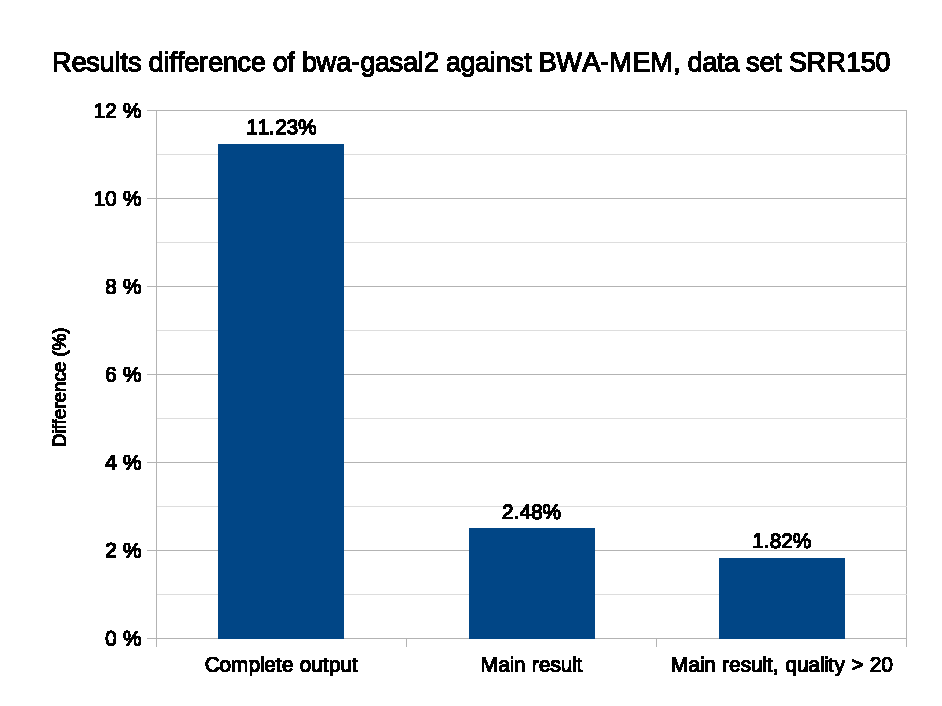
\includegraphics[width=1\linewidth]{srr150/score-check}
	\caption{Difference in the result with the mainline version of BWA}
	\label{fig:result-diff-srr150}
\end{figure}

We notice that the seed-only paradigm globally introduces a noticeable number of differences. 11.23\% of the lines are not matching. Many of the differences are due to reordering of the secondary results. Still, when we set aside the secondary results, which are mostly neglected in downstream analysis, this percentage drops to 2.48\%. Finally, when we remove low quality scores, the number of differences goes down to 1.82\%. Again, this small difference can come from seed filtering heuristics, as well as the seed-only paradigm itself. This threshold of 20 for the quality score is the usual value taken for downstream analysis. This is small enough to consider it acceptable.


